\documentclass{beamer}
\usepackage{graphicx} % Required for inserting images
\usepackage{booktabs}
\usepackage{hyperref}
\hypersetup{
    urlcolor=cyan,
    linkcolor=white,
    pdftitle={V0 Projet},
    pdfpagemode=FullScreen,
    }
\usepackage{float}
\usepackage{listings}
\usepackage{amsmath}
\usepackage{array}
\usepackage[french]{babel}
\usetheme{CambridgeUS}
\newcommand\Includegraphics[2][]{%
  \raisebox{-.5\dimexpr\height-\ht\strutbox+\dp\strutbox}{\includegraphics[#1]{#2}}}

\title{BDR Thermea: Modèle 3D d'une hélice toroïdale}
\author{Sacha Alidadi Heran}
\date{Novembre 2023}

\begin{document}

\maketitle

\section{Contexte et objectif}

\begin{frame}{Contexte}
    \begin{itemize}
        \item Les ingénieurs de BDR Thermea France, en particulier ceux du département simulation, ont besoin d'un modèle 3D d'une hélice toroïdale
        \item Le but est de pouvoir tester ce modèle dans un logiciel de simulation afin de voir s'il fait moins de bruit que le modèle actuel
        \item Une étude du MIT a montré que ce type d'hélice permet de réduire le bruit tonal pour des hélices de drone \href{https://news.mit.edu/2018/bladeless-turbine-drone-0612}{[1]}
    \end{itemize}
\end{frame}

\begin{frame}{Forme toroïdale}
    \begin{columns}[T]
        \hfill
        \begin{column}{.32\textwidth}
            \hspace{2mm}\Includegraphics[height=0.3\textheight]{images/ToroidalPropeller.png}\\
        \end{column}
        \hfill
        \begin{column}{.70\textwidth}
            \Includegraphics[height=0.4\textheight]{images/NormalVSToroidal.png} \hspace{2mm}\\
        \end{column}
        \hfill
    \end{columns}
\end{frame}

\begin{frame}{Objectifs}
    \begin{itemize}
        \item Établir les équations paramétriques de la courbe guide ainsi que les profils transverses.
        \item Générer la courbe guide et les profils transverses sur SALOME.
    \end{itemize}
\end{frame}

\begin{frame}{Contraintes}
    \begin{itemize}
        \item Il y a très peu de littérature sur les hélices toroïdales. Nous allons donc trouver les équations paramétriques nous même.
        \item Si nous ne trouvons pas d'équations, nous devrons adopter une approche CAO.
    \end{itemize}
\end{frame}

\begin{frame}{Modifications de la roadmap}
    \begin{itemize}
        \item Suite aux contraintes, nous avions initialement prévu de consacrer autant de temps à la recherche d'une équation paramétrique qu'à la génération de la courbe guide et des profils transverses sur SALOME.
        \item Les premières semaines nous ont montré que nous devions consacrer plus de temps à la recherche d'une équation paramétrique.
        \item Du au manque de temps, nous avons finalement avisé et décidé de consacrer plus de temps à la génération de la courbe guide et des profils transverses sur SALOME.
    \end{itemize}
\end{frame}

\section{Contributions}

\begin{frame}{Équations paramétriques d'une hélice toroidale d'un bateau}
    \begin{figure}
        \centering
        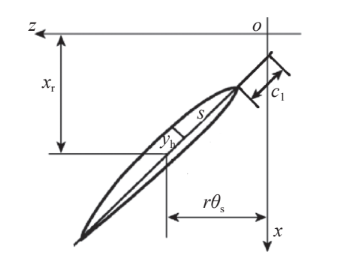
\includegraphics[scale=1]{images/ProfilTransverse.png}
        \caption{Profil transverse d'une pale}
    \end{figure}
\end{frame}

\begin{frame}{Équations paramétriques d'une hélice toroidale d'un bateau}
    \begin{alertblock}{Équation paramétrique de la courbe guide}
        \begin{equation*}
            \begin{cases}
                x = l + x_T +\left( \frac{-b}{2}+s \right) \sin\beta + \begin{pmatrix}
                    y_b \\
                    y_f
                \end{pmatrix} \cos\beta \\
                r = r_l \\
                \theta = \phi + \theta_s + \frac{1}{r} \left[ \left( \frac{-b}{2}+s \right) \cos\beta + \begin{pmatrix}
                    y_b \\
                    y_f
                \end{pmatrix} \sin\beta \right]
            \end{cases}
        \end{equation*}
    \end{alertblock}
\end{frame}

\begin{frame}
    \begin{alertblock}{Explication du paramètre $x_T$}
            \[ x_T(r) = x_l(r)+r \theta_s(r) \tan \beta(r) \]
    \end{alertblock}
\end{frame}

\begin{frame}{Forme de la courbe guide}
    \begin{figure}
        \centering
        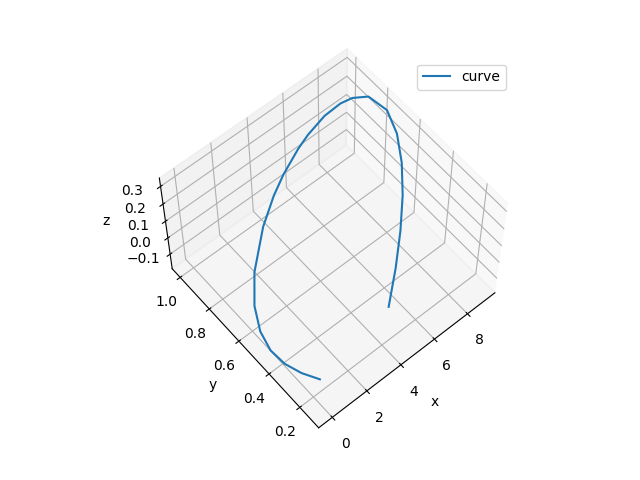
\includegraphics[scale=0.5]{images/Curve1D.png}
        \caption{Forme de la courbe guide}
    \end{figure}
\end{frame}

\begin{frame}{Equation paramétrique du profil transverse}
    \begin{alertblock}{Equation du profil}
        \begin{equation*}
            \begin{cases}
                x(t) = x_l + r \theta_s + \tan(\beta) \\
                y(t) = r \cos(\theta) \\
                z(t) = r \sin(\theta)
            \end{cases}
        \end{equation*}
    \end{alertblock}
\end{frame}

\begin{frame}{Illustration du profil transverse}
    \begin{figure}
        \centering
        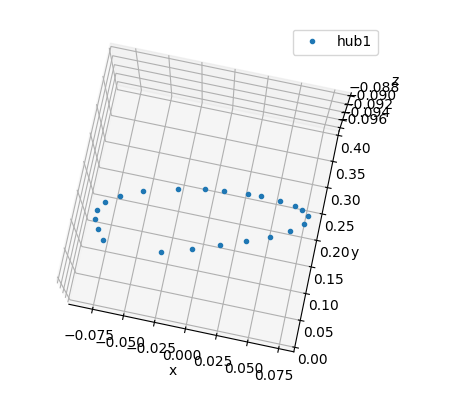
\includegraphics[scale=0.5]{images/Transverse_profile_fan_chinese_paper.png}
        \caption{Profil transverse à partir des équations précédentes}
    \end{figure}
\end{frame}

\begin{frame}{Génération des hélices sur SALOME}
    \begin{itemize}
        \item Pour générer les hélices sur SALOME, il suffit d'extruder le profil transverse le long de la courbe guide.
        \item Il suffit de générer une seule pale pour générer l'hélice complète.
        \item Il faut faire attention aux éventuelles intersections entre les pales.
    \end{itemize}
\end{frame}

\begin{frame}{Modèle 3D de l'hélice}
    \begin{figure}
        \centering
        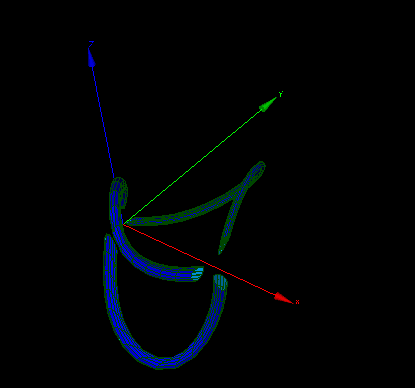
\includegraphics[scale=0.5]{images/ToroidalPropellerBoat.png}
        \caption{Génération de l'hélice sur SALOME}
    \end{figure}
\end{frame}

\begin{frame}{Variante projetée de l'hélice}
    \begin{figure}
        \centering
        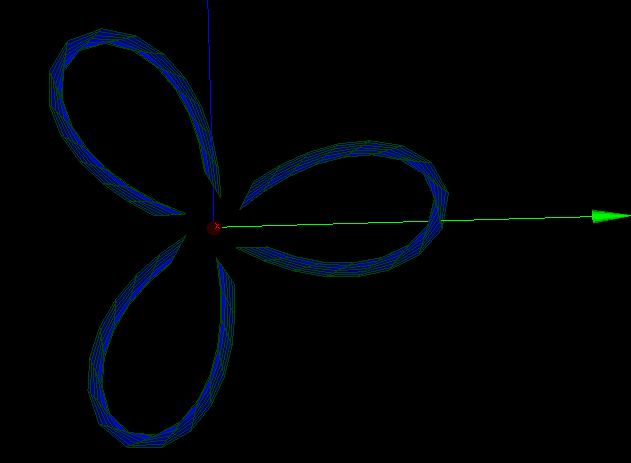
\includegraphics[scale=0.5]{images/ToroidalPropellerBoatProjected.png}
        \caption{Variante de l'hélice dont les courbes guides ont été projetées sur le plan $0yz$}
    \end{figure}
\end{frame}

\begin{frame}{Avantages et inconvénients de ce modèle}
    \begin{itemize}
        \item Avantages
        \begin{itemize}
            \item Facile à générer
            \item Possibilité de générer des hélices avec des profils NACA
        \end{itemize}
        \item Inconvénients
        \begin{itemize}
            \item Difficile de varier les paramètres
            \item Les profils transverses ne sont pas assez larges pour notre ventilateur
        \end{itemize}
    \end{itemize}
\end{frame}

\begin{frame}{Hélice toroidale en CAO}
    \begin{itemize}
        \item Durant le projet, nous avons portés notre attention sur la génération d'une hélice entièrement en CAO
        \item Nous nous sommes basés sur ce modèle d'hélice \href{https://github.com/RaulBejarano/Ultimate-Toroidal-Propeller-Generator}{[2]}
    \end{itemize}
\end{frame}

\begin{frame}{Visualisation de l'hélice}
    \begin{figure}
        \centering
        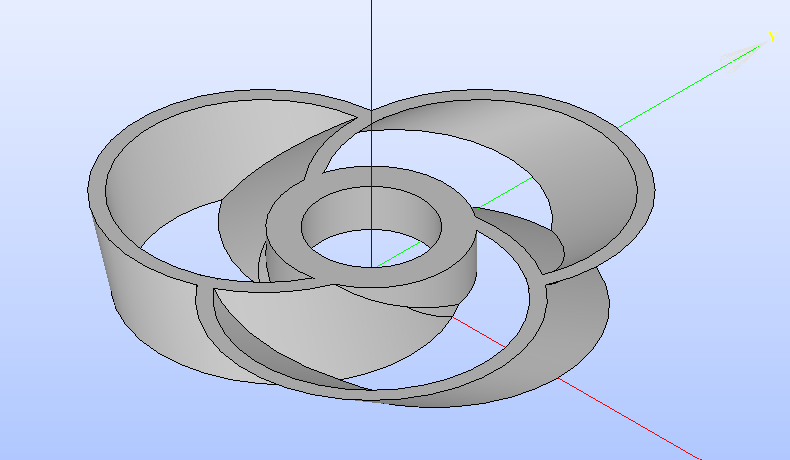
\includegraphics[scale=0.5]{images/ToroidalPropellerCAD.png}
        \caption{Modèle d'hélice toroïdale en CAO}
    \end{figure}
\end{frame}

\begin{frame}{Avantages et inconvénients}
    \begin{itemize}
        \item Avantages
        \begin{itemize}
            \item Facile à générer
            \item Les intersections entre les hélices sont facilement automatisables
        \end{itemize}
        \item Inconvénients
        \begin{itemize}
            \item On ne peut pas varier les paramètres
            \item Les profils transverse n'ont pas un profil NACA
        \end{itemize}
    \end{itemize}
\end{frame}

\begin{frame}{Équations paramétriques d'une hélice toroidale adaptée à une pompe à chaleur}
    \begin{itemize}
        \item Au milieu du projet, nous avons consacré tout notre temps sur l'établissement d'équations paramétriques de courbes guides.
        \item Nous nous sommes basés sur des courbes déjà existantes.
        \item Parmi ces courbes, nous avons choisi la trifolium.
    \end{itemize}
\end{frame}

\begin{frame}{Équation de la trifolium}
    \begin{alertblock}{Équation paramétrique de la courbe guide}
        \begin{equation*}
            \begin{cases}
                x(t) = \cos(2t) - \cos(t) \\
                y(t) = \sin(2t) + \sin(t)
            \end{cases}
        \end{equation*}
    \end{alertblock}
\end{frame}

\begin{frame}{Visualisation de la trifolium}
    \begin{figure}
        \centering
        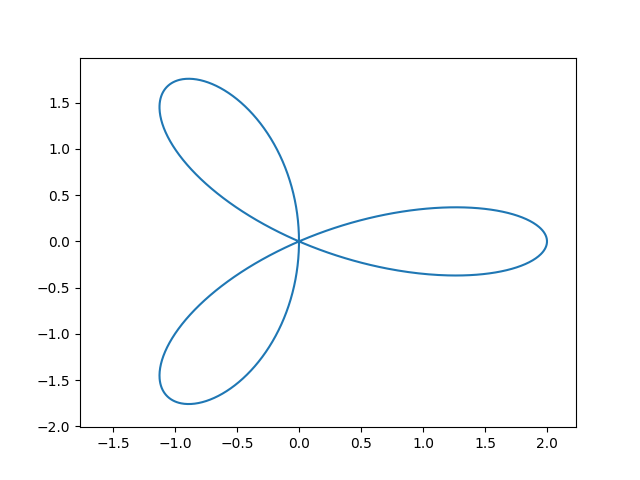
\includegraphics[scale=0.5]{images/Trifolium.png}
        \caption{Trifolium}
    \end{figure}
\end{frame}

\begin{frame}{Généralisation 3D de la trifolium}
    \begin{alertblock}{Équation paramétrique de la courbe guide}
        \begin{equation*}
            \begin{cases}
                x(t) = \cos((N-1)t) - \cos(t) \\
                y(t) = \sin((N-1)t) + \sin(t) \\
                z(t) = \sin(Nt)\theta + \left\{ \frac{t N}{2\pi} \right\} L
            \end{cases}
        \end{equation*}
    \end{alertblock}
\end{frame}

\begin{frame}{Génération d'un profil transverse 3D}
    \begin{alertblock}{Courbe de la bielle de Bérard}
        \begin{equation*}
            \begin{cases}
                x(\theta) = b \cos(\theta) + kd(\theta) - l\epsilon \sqrt{c^2 - d^2(\theta)} \\
                y(\theta) = b \sin(\theta) + k \epsilon \sqrt{c^2 - d^2(\theta)} + ld(\theta)
            \end{cases}
        \end{equation*}
    \end{alertblock}
    \begin{alertblock}{Explication du terme $d(t)$}
        \[ d(\theta) = a-b\cos(\theta) \]
    \end{alertblock}
\end{frame}

\begin{frame}{Visualisation de la courbe de la bielle de Bérard}
    \begin{figure}
        \centering
        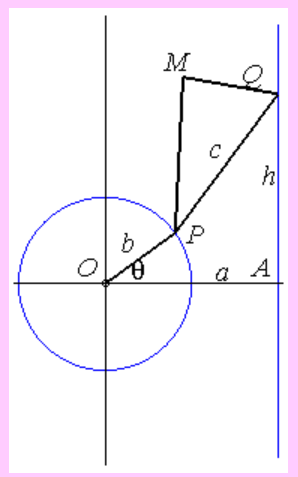
\includegraphics[scale=0.5]{images/SliderCrankMechanismCurve.png}
        \caption{Illustration de la bielle de Bérard}
    \end{figure}
\end{frame}

\begin{frame}{Résultats générés sur SALOME}
    \begin{figure}
        \centering
        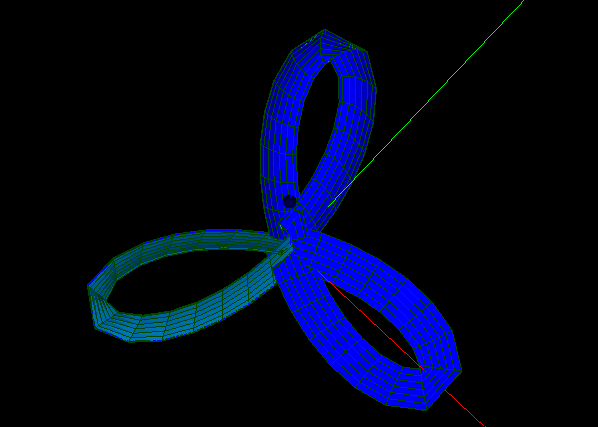
\includegraphics[scale=0.5]{images/ParametricEquation-L0-T0.png}
        \caption{Hélice toroïdale générée sur SALOME}
    \end{figure}
\end{frame}

\begin{frame}{Résultats générés sur SALOME}
    \begin{figure}
        \centering
        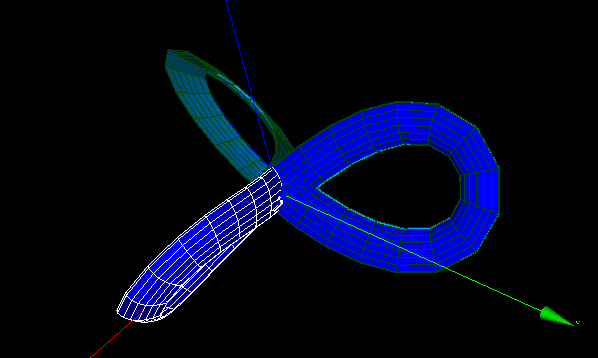
\includegraphics[scale=0.5]{images/ParametricEquation-L0-T0p5.png}
        \caption{Hélice toroïdale générée sur SALOME}
    \end{figure}
\end{frame}

\begin{frame}{Résultats générés sur SALOME}
    \begin{figure}
        \centering
        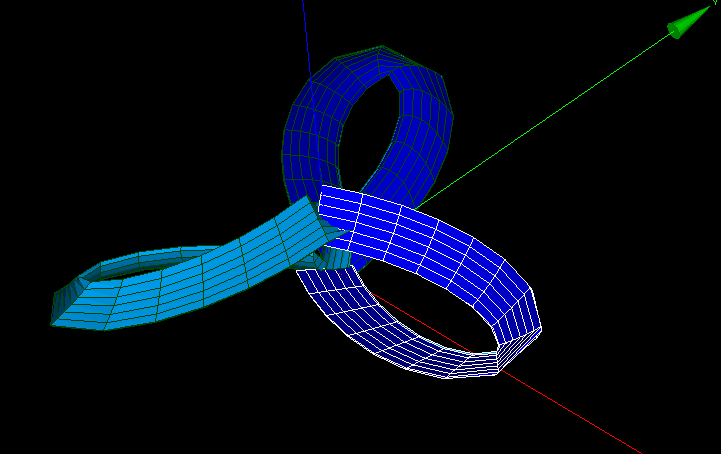
\includegraphics[scale=0.5]{images/ParametricEquation-L0p5.png}
        \caption{Hélice toroïdale générée sur SALOME}
    \end{figure}
\end{frame}

\begin{frame}{Résultats générés sur SALOME}
    \begin{figure}
        \centering
        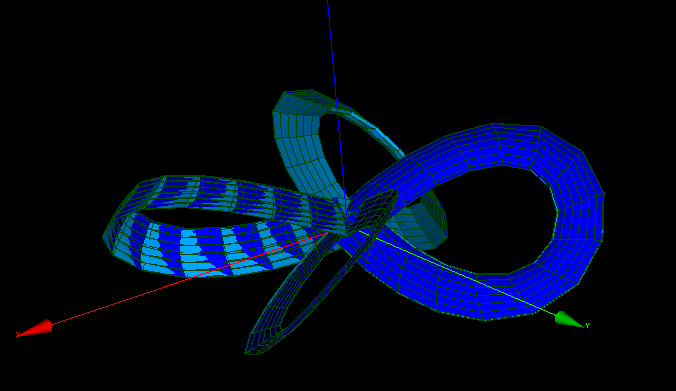
\includegraphics[scale=0.5]{images/ParametricEquation-L0-T0-B4.png}
        \caption{Hélice toroïdale générée sur SALOME}
    \end{figure}
\end{frame}

\begin{frame}{Avantages et inconvénients}
     \begin{itemize}
        \item Avantages
        \begin{itemize}
            \item Facile à générer
            \item Possibilité de varier les paramètres
        \end{itemize}
        \item Inconvénients
        \begin{itemize}
            \item Difficile de varier la largeur des pales
            \item Les intersections entre les hélices doivent être gérées au cas pas cas
        \end{itemize}
     \end{itemize}
\end{frame}

\begin{frame}{Hélice toroidale adaptée à une pompe à chaleur en CAO}
    \begin{alertblock}{Ce qu'il faut pour générer l'hélice}
        \begin{itemize}
            \item Une courbe guide
            \item Un profil de départ et d'arrivée
            \item Des profils transverses intermédiaires
        \end{itemize}
    \end{alertblock}
\end{frame}

\begin{frame}{Résultats souhaités}
    \begin{figure}
        \centering
        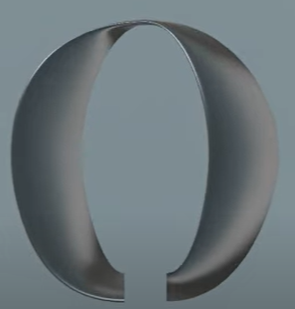
\includegraphics[scale=0.5]{images/Large_Toroidal.png}
        \caption{Résultat souhaité: Un bout de pale fin et le milieu de la pale large}
    \end{figure}
\end{frame}

\begin{frame}{Résultats générés sur SALOME}
    \begin{figure}
        \centering
        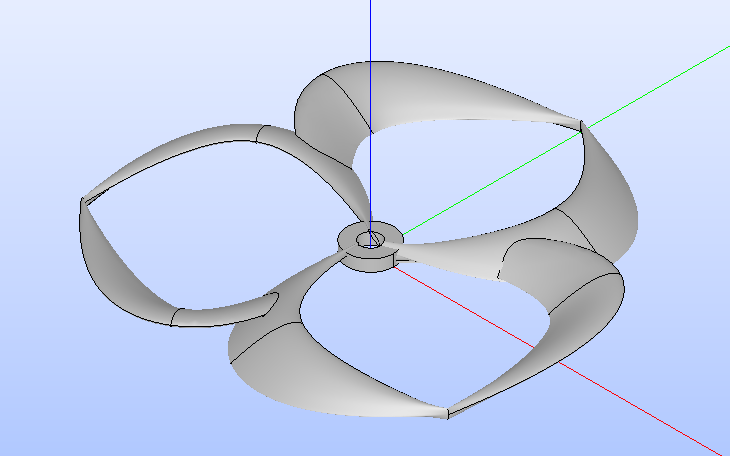
\includegraphics[scale=0.5]{images/ToroidalNACAcad.png}
        \caption{Résultat obtenu sur SALOME: Le modèle a des irrégularités}
    \end{figure}
\end{frame}

\begin{frame}{Résultats corrigées sur SALOME}
    \begin{figure}
        \centering
        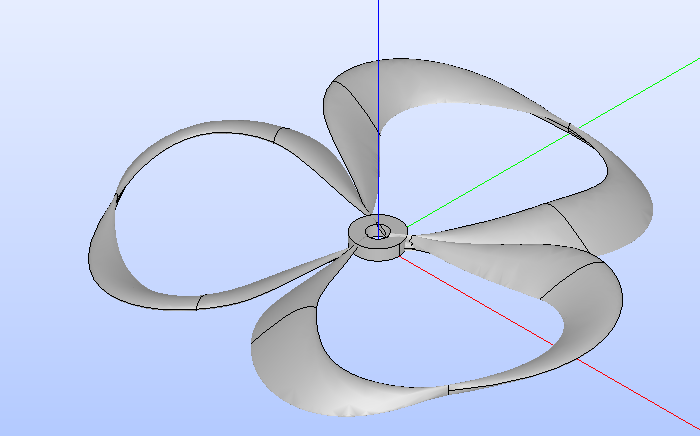
\includegraphics[scale=0.5]{images/ToroidalNACAcad_Smooth.png}
        \caption{Résultat obtenu sur SALOME: Le modèle n'a plus d'irrégularités au bout de la pale}
    \end{figure}
\end{frame}

\begin{frame}{Résultat final}
    \begin{figure}
        \centering
        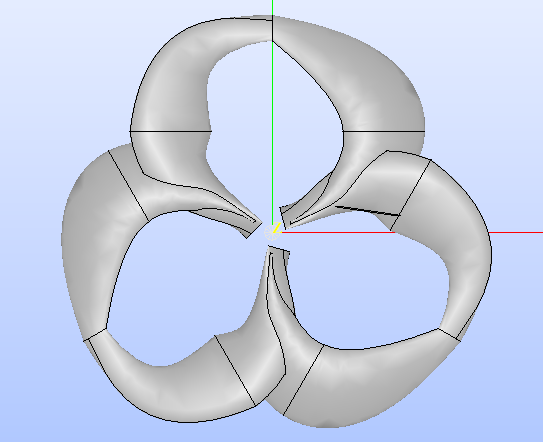
\includegraphics[scale=0.5]{images/CAD_Normal.png}
        \caption{Résultat obtenu sur SALOME: Le modèle a moins d'irrégularités que ces prédecesseurs}
    \end{figure}
\end{frame}

\begin{frame}{Avantages et inconvénients}
    \begin{itemize}
        \item Avantages
        \begin{itemize}
            \item Possibilité de varier les paramètres
            \item Possibilité de varier la largeur des pales
        \end{itemize}
        \item Inconvénients
        \begin{itemize}
            \item Irrégularités autour du ventilateur
            \item Les intersections entre les hélices doivent être gérées au cas pas cas
        \end{itemize}
    \end{itemize}
\end{frame}

\section{Conclusion}

\begin{frame}{Pistes d'amélioration}
    \begin{itemize}
        \item Travailler sur une nouvelle équation de courbe guide qui permet de varier la largeur des pales
        \item Lisser les irrégularités autour du ventilateur
    \end{itemize}
\end{frame}

\begin{frame}{Bilan}
    \begin{itemize}
        \item Nous avons réussi à créer des modèles d'hélices toroïdales.
        \item Les modèles générés sur SALOME présentes toujours des irrégularités à corriger.
    \end{itemize}
\end{frame}

\end{document}